\begin{frame}
  \frametitle{Projet CASSIS}
  \begin{block}{Cadre du projet}
    Projet de deuxième année informatique sur 6 mois à l'Enseirb-Matmeca sur la simulation de caches.\\
    Client : Denis Barthou, INRIA et Enseirb-Matmeca\\
    Responsable : Floréal Morandat, LaBRI et Enseirb-Matmeca
  \end{block}
  \begin{block}{A quels besoins répond le projet CASSIS ?}
  \begin{itemize}  
  \item Rejouer une exécution mutli-threadée d'un programme donné
  \item Architecture libre des caches
  \item Gestion configurable des politique de caches 
  \item Réutilisation possible du code
  \end{itemize}
  \end{block}
\end{frame}

\begin{frame}
  \frametitle{Outils existants d'étude de caches}
  \begin{block}{Papi}
  \begin{itemize}
    \item Compteur hardware
    \item Paramètres difficillement simulables
    \end{itemize}    
  \end{block}
  \begin{block}{Cachegrind}
    \begin{itemize}
    \item Simulation d'un thread
    \item Exécution séquentielle
    \end{itemize}
  \end{block}   

  \begin{block}{Intérêts d'une simulation}
    \begin{itemize}
        \item Architecture libre
        \item Choix des politiques
    \end{itemize}
  \end{block}
\end{frame}



\begin{frame}
  \frametitle{Autour de CASSIS}
  \begin{figure}
    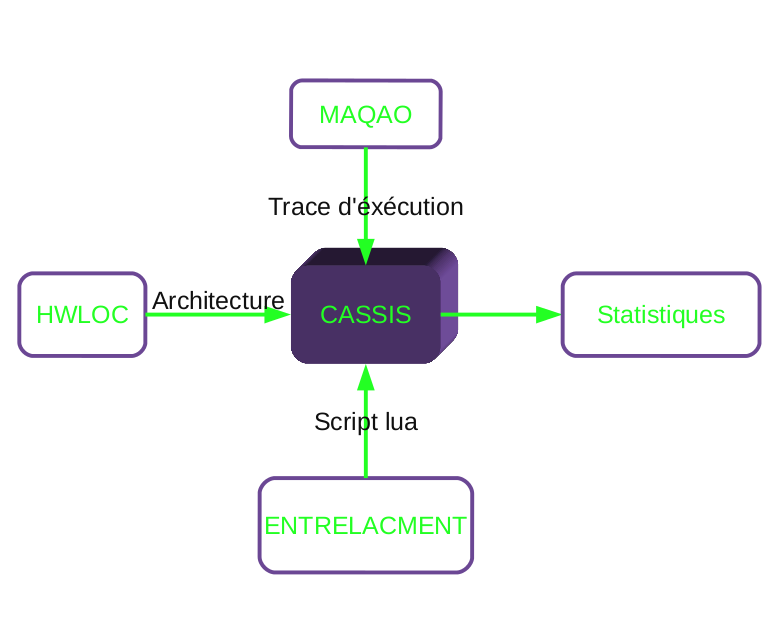
\includegraphics[scale=0.4]{images/schema_cassis.png}
  \end{figure}
\end{frame}
